\chapter{Kryptologie}
Die Kryptologie ist die Wissenschaft der Verschlüsseln. Sie wird unterteilt in:
\begin{itemize}
	\item \textbf{Kryptographie:} Verschlüsseln und Entschlüsseln
	\item \textbf{Kryptoanalyse:} kryptographische Verfahren berechnen
\end{itemize}

\subsection*{Wozu dient Verschlüsselung?}
Es wird Verschlüsselt um das Ziel der \textbf{Confidentiality (Vertraulichkeit)} zu erreichen. Die asymmetrische Kryptographie kann aber auch zum Erlangen von Authentizität und Nichtabstreitbarkeit verwendet werden.

\subsection*{Wie funktioniert Verschlüsselung?}
\textit{Alice} möchte eine Nachricht (Klartext) an \textit{Bob} schicken, ohne dass unberechtigte Zuhörer wie \textit{Eve} den Chiffretext nicht verstehen. 
\begin{figure}[H]
	\centering
	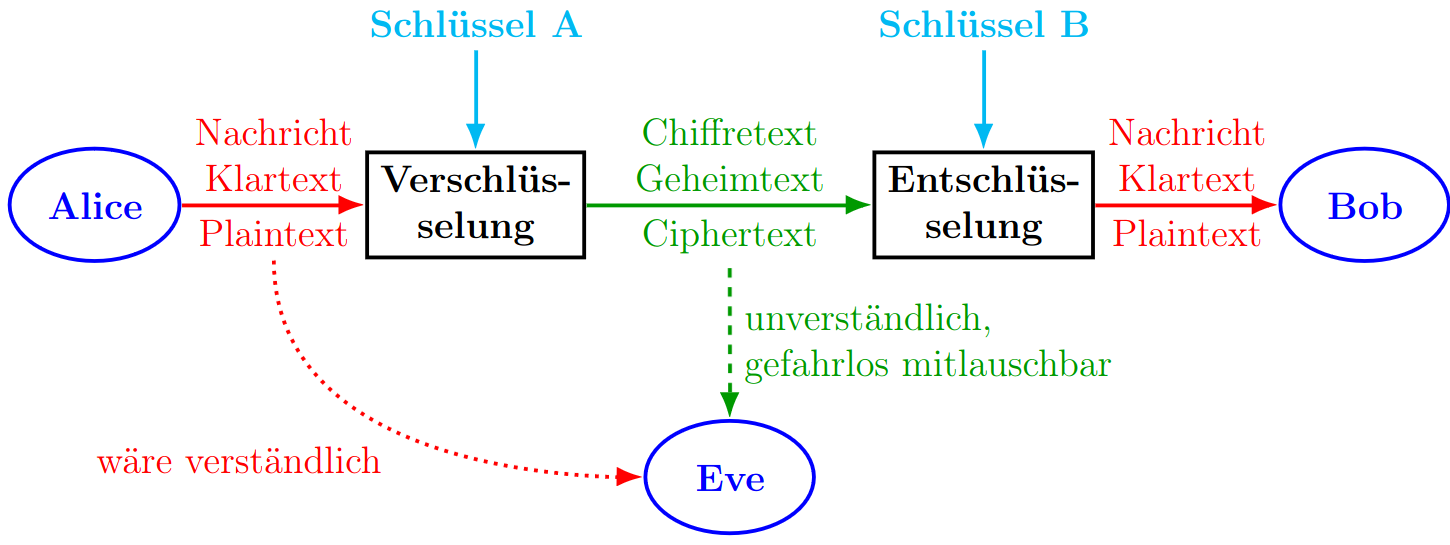
\includegraphics[width=1.0\linewidth]{figures/verschallg.png}
	\caption{Grundlegende Situation der verschlüsselten Kommunikation}
\end{figure}
Die Daten werden so verändert, dass sie für \textit{Eve} nicht rekonstruierbar sind, für \textit{Bob} aber schon. Daher benötigen \textit{Alice} und \textit{Bob} für das Ver- und Entschlüsseln der Nachricht einen Schlüssel.


\subsection*{Geschichtliche Einordnung}
Der Wunsch, militärische, politische oder persönliche Geheimnisse vor Unbefugten zu schützen, ist mit Sicherheit alt. Einfache Verfahren dazu sind z.B. von Caesar bekannt. Es gab neuzeitlich Verfahren, die sich lange Analyse widersetzten (z.B. Vigenère). 

Während des 1. und 2. Weltkrieges wurde die Kommunikation zwischen den Truppen verschlüsselt, mitgehört, geknackt, anders verschlüsselt, usw. Im 2. Weltkrieg wurde erstmals MathematikerInnen miteinbezogen (England: Alan Turin, Analyse von Enigma). Im Gegensatz zu früher, als die Kryptoanalyse eher von SprachwissenschaftlerInnen betrieben wurde, wird sie heute von InfromatikerInnen und MathematikerInnen durchgeführt.

Früher war der Bedarf von Verschlüsselung für Herrschende und Regierungen vermutlich höher als für Privatpersonen. Heutzutage ist sie aber auch für Privatpersonen wichtig.

Die Zeit der asymmetrischen Kryptosystemen, die das Schlüsselaustauschproblem lösten, begann 1976. Mit ihnen wurde es möglich, dass 2 Personen über das Internet abhörsicher kommunizieren können.

\subsection*{Wie wird die Unverständlichkeit für Eve erreicht?}
Früher wurde vor allem darauf gesetzt, dass Unbefugten das Verfahren selbst unbekannt war. Dies hat viele Nachteile:
\begin{itemize}
	\item Funktioniert zwischen zwei Verfeindeten Fraktionen (Freund-Feind-Schema), aber nicht wenn 2 Personen kommunizieren wollen, da man für jedem ein eigenes Verfahren benötigen würde
	\item Entwicklung und Beibringen von neuen Verfahren ist aufwendig
	\item Die Geheimhaltung des Verfahrens ist, besonders bei großen Maßstäben, schwierig (Verreden, Gefangennahme, Folter, Bestechung, Drohung).
	\item Selbst entwickelte Verfahren haben mit hoher Wahrscheinlichkeit Schwachstellen. Moderne Verfahren sind öffentlich bekannt und seit Jahrzenten erforscht, analysiert und diskutiert.
\end{itemize}

Daher folgen heute anerkannte Verfahren (DES, AES, RSA,...) dem \textbf{Prinzip von Kerkhoff:} \textit{''Das Verfahren darf nicht der Geheimhaltung bedürfen und soll ohne Schaden in Feindeshand fallen können.''} 

Moderne Verfahren sind so sicher, dass sie vor Angriffen sicher sind, auch wenn die Angreifer das Verfahren kennen. Die Sicherheit liegt in der Geheimhaltung des Schlüssels.

Schlüssel lassen sich leichter erzeugen, verbreiten und geheimhalten als Verfahren. Außerdem kann man für Kommunikation mit mehreren Personen einfach verschiedene Schlüssel verwenden.

\subsection*{Key Management}
Auch wenn es einfacher ist den Schlüssel als wie das Verfahren geheimzuhalten, ist das Key Management heikel. Hier geht es um das Erzeugen von Schlüsseln, ihren Austausch, Speicherung, Nutzung und Vernichtung. Moderne Chiffren sind so gut entworfen, dass Attacken meist auf Social Engineering, Seitenkanalangriffe oder am Key Management basieren.

\subsection*{Wie hört Eve überhaupt ab?}
Aus Glasfaserkabeln wird Licht gestreut \\
Bei WLAN und anderen drahtlosen Übertragungen: Broadcast $\rightarrow$ Frequenzen \\
Weiter Möglichkeiten sind Man-in-the-Middle Angriffe, DNS/DHCP/ARP-Spoofing

